\chapter{随机实验中费希尔推断与内曼推断的统一}\label{chapter::unification-fisher-neyman}
 \chaptermark{费希尔推断与内曼推断的统一}


第\ref{ch::frt-cre}至\ref{chapter::mpe}章介绍了不同实验中的 Fisher 推断与 Neyman 推断。Fisher 视角检验任何单位都不存在因果效应的强零假设，关注有限样本精确$p$值；Neyman 视角关注平均因果效应的无偏估计及保守大样本置信区间。二者都由实验设计保证的实际随机化支持，因而都称为{\it 基于随机化的推断}或{\it 基于设计的推断}。由于讨论实验中有限总体的单位，也称为{\it 有限总体推断}。它们既相互联系，也各具特点。 

1935年，内曼向英国皇家统计学会提交了关于基于随机化推断的开创性论文。他的论文\citep{neyman1935statistical}在讨论环节遭到了费希尔的批驳。\cite{sabbaghi2014comments}回顾了这场著名的内曼-费希尔之争，并就该经典问题给出了新的研究结果。本章并不深究其中的哲学争议，而旨在提供一种统一的讨论框架。 



\section{在CRE中检验强零假设与弱零假设} 
 \label{sec::strong-weak-cre-frt}
 
 
重新考虑处理—对照完全随机实验。Fisher 视角检验强零假设
$$
\HF: Y_i(1) = Y_i(0) \text{ for all units } i=1,\ldots, n.
$$
FRT 给出\eqref{eq::exactpvalue}定义的有限样本精确$p_\frt$。 
 
 
由置信区间与假设检验的对偶性，Neyman 视角根据
$$
t= 
\frac{\hat{\tau} }{  \sqrt{  \hat{V}    } }  .
$$
检验弱零假设
$$
\HN : \tau = 0  \Longleftrightarrow \HN: \bar{Y}(1) = \bar{Y}(0)
$$
由$\hat\tau$的中心极限定理及方差估计的保守性，
$$
t  =   \sqrt{  \frac{ \var(\hat{\tau}) }{ \hat{V} } } \times  \frac{\hat{\tau} }{  \sqrt{  \var(\hat{\tau})   } }    \rightarrow  C \times   \N01 
$$
依分布收敛，其中$C$不大于$1$，但依赖未知潜在结果。将学生化统计量$t$与$\N01$的分位点比较，可得$\HN$的保守大样本检验。 

此外，\citet{ding2017randomization}证明：使用学生化统计量$t$开展FRT时具有双重保障：
\begin{enumerate}
\item 
 在强零假设$\HF$成立时，$p_\frt$值为有限样本精确值；
\item
 在弱零假设$\HN$成立时，$p_\frt$值具有大样本保守性。
\end{enumerate}
这种特性仅存在于学生化统计量$t$中。\citet{ding2017randomization}还指出：若采用其他统计量进行FRT，则未必能获得上述双重保障；特别是使用$\hat{\tau}$作为统计量时，在$\HN$成立条件下可能会出现大样本反保守性现象。以下我将通过理论分析阐释学生化操作在FRT中的必要性。 


在$\HN$下，有
$$
\hat{\tau} \asim \textsc{N}\left(0,    \frac{S^2(1)}{n_1} + \frac{S^2(0)}{n_0} -  \frac{S^2(\tau)}{n}    \right).
$$
FRT 假装科学表为$\HF$所规定的$(Y_i, Y_i)_{i=1}^n$，因此$\hat{\tau} $的随机化分布为
$$
(\hat{\tau} )^\pi \asim \textsc{N}\left(0,    \frac{s^2}{n_1} + \frac{s^2}{n_0}    \right),
$$
其中$(\cdot)^\pi$表示随机化分布。\footnote{$\pi$是表示随机置换的标准记号。}
$
s^2 
$
是观测结果的样本方差。根据第\ref{ch::frt-cre}章的\eqref{eq::frt-algebra-difference-in-means}，可将$\HF$下$(\hat{\tau} )^\pi$的渐近方差近似为
\begin{eqnarray*}
\frac{s^2}{n_1} + \frac{s^2}{n_0} 
& =& \frac{n}{n_1 n_0}  \left\{ 
 \frac{n_1 -1}{ n-1 } \hat S^2(1) + \frac{n_0 - 1}{n-1} \hat S^2(0) + \frac{n_1n_0}{n(n-1)} \hat\tau^2
 \right\} \\
&\approx & \frac{\hat S^2(1) }{n_0} +  \frac{\hat S^2(0) }{n_1} \\ 
&\approx & \frac{  S^2(1) }{n_0} +  \frac{  S^2(0) }{n_1},
\end{eqnarray*}
它不等于$\hat{\tau} $的渐近方差。理想情况下，检验$\HN$的$p$值应根据$\hat{\tau} $的真实分布计算，但它依赖未知潜在结果。FRT 则使用置换分布$(\hat{\tau} )^\pi $计算$p_\frt$，即使在大样本下也不等于$\HN$下$\hat{\tau} $的真实分布。因此，以$\hat\tau$作 FRT，即使大样本也未必控制$\HN$下的第一类错误率。 
 
 
幸运的是，将原统计量$\hat{\tau} $改为学生化版本$t$，就能消除以$\hat\tau$作 FRT 的上述问题。在$\HN$下，
$$
t \asim \textsc{N}(0,  C^2)
$$
其中$C^2 \leq 1$，且所有单位$i=1, \ldots, n$满足$Y_i(1) - Y_i(0) = \tau$时取等号。FRT 假装所有$i$都满足$Y_i(1) = Y_i(0) = Y_i$，生成置换分布
$$
t^\pi \asim \textsc{N}(0,  1)
$$
方差为$1$，因为 FRT 使用的科学表中个体因果效应均为零。在$\HN$下，$t$的真实分布比对应置换分布更集中，因此基于$t$的$p_\frt$渐近保守。 

%Whether $\HF$ or $\HN$ makes more sense? This is a famous controversy between Neyman and Fisher in a meeting at the Royal Statistical Society, UK \citep{neyman1935statistical, sabbaghi2014comments, Ding:2014}.  
%Recently, \citet{ding2017randomization} advocated using $\hat{\tau} /  \sqrt{  \hat{V}    } $, i.e., the studentized statistic $t$ in Example \ref{eg::studentized-statistic} of Chapter \ref{ch::frt-cre}, in the FRT so that the $p$-value is finite sample exact for $\HF$ and asymptotically valid for $\HN$.  In contrast, using the difference-in-means in the FRT does not have these guarantees. 







 
 
\section{CRE中的协变量校正型FRT}
 \label{sec::xfrt-cre}
 
将第\ref{sec::strong-weak-cre-frt}节推广到含协变量的情形，\citet{zhao2020caFRT}建议以学生化的\citet{lin2013}估计量进行 FRT：
$$
t_\textsc{L}   =  \frac{  \hat{\tau}_\textsc{L} }{  \sqrt{\hat{V}_\textsc{L}}  },
$$
它是将$Y_i$对$( 1, Z_i, X_i, Z_i X_i) $作 OLS 回归时，$Z_i$系数的稳健$t$统计量。他们证明，以$t_\textsc{L} $作 FRT 具有多重保证：
 \begin{enumerate}
\item
 在强零假设$\HF$条件下，$p_\frt$具有有限样本精确性；
\item
 在弱零假设$\HN$条件下，$p_\frt$具备大样本保守性；
\item
 当$\HN$不成立且协变量能预测结果时，$p_\frt$对应检验的渐近功效高于基于$t$的 FRT；
\item
即便线性结果模型设定存在偏差，上述特性依然成立。 
\end{enumerate}
这同样是学生化统计量$t_\textsc{L} $的特性。\citet{zhao2020caFRT}证明，第\ref{sec::covariate-adjusted-frt-intro}节的其他协变量调整 FRT，可能在$\HN$下反保守，或在$\HN$不成立时功效低于基于$t_\textsc{L} $的 FRT。  




\section{模拟研究}
\label{sec::simulation-xfrt-typeoneerror}




下面通过模拟评价弱零假设下各$p_\frt$的有限样本性质，使用以下十二种统计量。
\begin{enumerate}
\item
前三种统计量源自内曼\citet{Neyman:1923}的OLS推导，依次为处理组系数、基于经典标准误的$t$统计量及基于EHW标准误的$t$统计量。

\item
接下来三个统计量采用定义\ref{def::pseudo-y-frt}的伪结果策略，\citet{rosenbaum2002covariance}倡导过该方法。先将$Y_i$对$(1,X_i)$回归，得到残差，再像前三个统计量一样构造统计量。

\item
接下来三个统计量基于\citet{fisher1925statistical}的 OLS 实现，见第\ref{sec::ancova}节。

\item
最后三种对应\citet{lin2013}的OLS推导，亦在第\ref{sec::ancova}章中探讨。
\end{enumerate}

 


考虑包含$n=100$个单位的有限总体，实施组别大小为$(n_1, n_0) =(20,80)$的完全随机实验。对每个$i  $，从 Unif$(-1,1)$抽取一元协变量$ X_i $，生成潜在结果$Y_i(1) \sim \textsc{N}(  X_i ^3 , 1)$和$Y_i(0) \sim \textsc{N}( - X_i ^3 , 0.5^2)$，再分别中心化各$Y_i(1)$与$Y_i(0)$，保证$\tau= 0$。模拟时固定$\{Y_i(1), Y_i(0),  X_i \}_{ i = 1}^{n} $，随机置换$n_1$个 1 与$n_0$个 0，得到观测结果并实施 FRT。重复 500 次，每次用处理向量的 500 次独立置换近似$p$值。 



图\ref{fig::xfrt-type1error}呈现了弱零假设下的$p$值分布。唯独底部四列稳健$t$统计量能维持第一类错误率在设定水平，且呈保守特性符合理论预期。其余八种统计量均导致第一类错误率超出名义水平，故不宜用于弱零假设检验。

 



\begin{sidewaysfigure} 
\centering
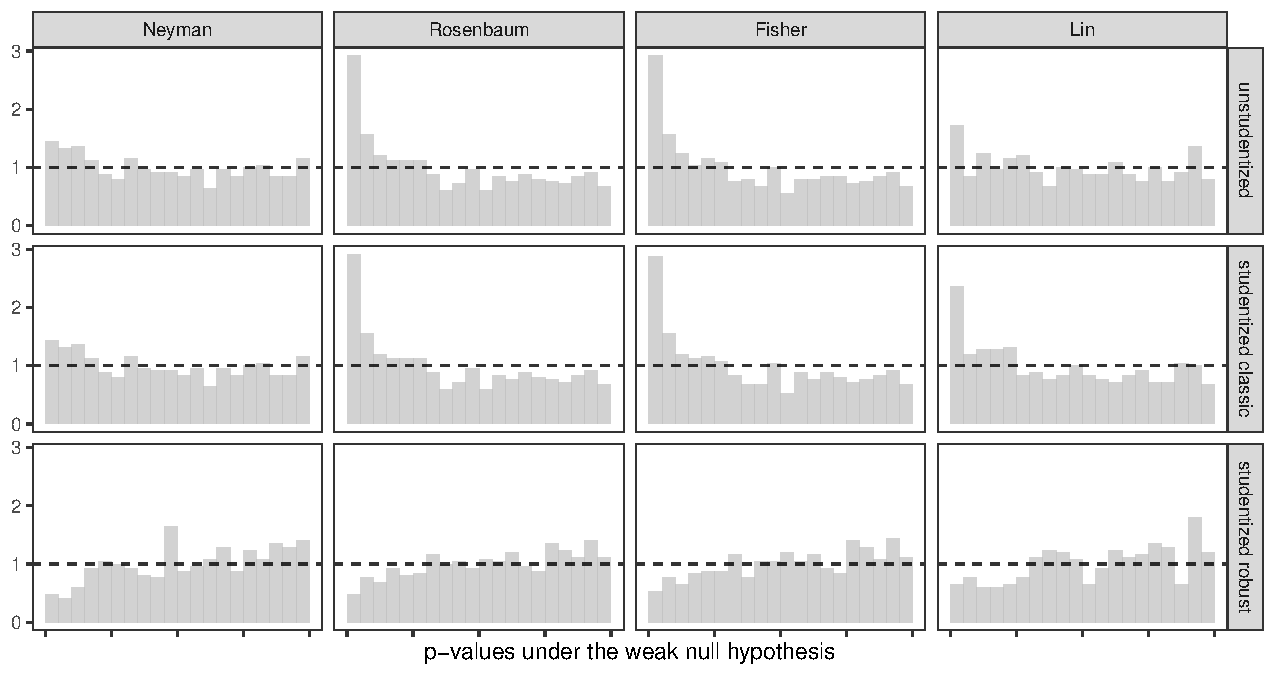
\includegraphics[width = \textwidth]{figures/typeoneerrorXFRT.pdf}
\caption{弱零假设下$p_\frt$值的直方图}\label{fig::xfrt-type1error}
\end{sidewaysfigure}










\section{综合建议}






若需同时检验强弱零假设，SRE场景下的建议与CRE相似。回顾第\ref{chapter::stratification-poststratification}章与\ref{sec::covariate-SRE}章的估计量：无协变量时\citet{zhao2020caFRT}推荐采用
$$
t_\textsc{S} =  \frac{  \hat{\tau}_\textsc{S} }{  \sqrt{\hat{V}_\textsc{S}} } ;
$$ 
存在协变量时则建议利用
$$
t_\textsc{L,S} =  \frac{  \hat{\tau}_\textsc{L,S} }{  \sqrt{\hat{V}_\textsc{L,S}} } . 
$$ 


再随机化的分析更微妙。\citet{zhao2020caFRT}证明，基于$t$的 FRT 不再具有第\ref{sec::strong-weak-cre-frt}节的双重保证，但基于$t_\textsc{L}$的 FRT 仍保有第\ref{sec::xfrt-cre}节的保证，说明再随机化下协变量调整与学生化都很重要。 




配对实验也有类似结论。不含协变量时，建议将$\hat\tau_i$仅对$1$作 OLS 回归，以截距的$t$统计量实施 FRT；含协变量时，将$\hat\tau_i$对$1$与$\hat\tau_{X,i}$回归，以截距的$t$统计量实施 FRT。第\ref{chapter::mpe}章图\ref{fig::frt-television-mpe}采用了这些推荐方法。 



总体上，以学生化统计量实施 FRT 是更稳妥的选择。若学生化统计量的大样本正态近似准确，$p_\frt$与正态近似$p$值几乎相同；若近似不准确，FRT 至少仍保证强零假设下$p$值有效。这就是本书的建议。 



\section{案例研究}
\label{sec::case-study-chong}

 

回顾第\ref{sec::ps-chong}节分析的\citet{chong2016iron}分层随机实验，分别比较“足球”组与“对照”组、“医生”组与“对照”组，并比较是否使用基线贫血状态协变量的 FRT。该数据可同时说明完全随机实验和分层随机实验的 FRT：同一年级内的十项亚组分析使用完全随机实验的$t$和$t_\textsc{L}$；对所有年级平均的两项总体分析使用分层随机实验的$t_\textsc{S}$和$t_\textsc{L,S}$。 

表\ref{tb::pv-values-chong}给出点估计、标准误、稳健$t$统计量正态近似的$p$值，以及 FRT 的$p$值。由于基线贫血能预测结果，多数层中协变量调整降低了标准误。表\ref{tb::pv-values-chong}也有两个例外：二年级比较“足球”与“对照”、四年级比较“医生”与“对照”时，调整后标准误增加。这是层内组别人数较少、渐近近似不准确所致，但两例的差异都仅在第三位数字。正态近似与 FRT 的$p$值很接近，后者多数略大。根据理论，应更信赖 FRT 的$p$值，因为它还有尖锐零假设下有限样本精确的额外保证。本例层内人数很少，这一点尤其重要。 

\begin{table}
\centering
\caption{基于\citet{chong2016iron}数据的再分析：“\textsc{N}”表示\citet{Neyman:1923}的不调整协变量估计与检验，“\textsc{L}”表示\citet{lin2013}的协变量调整估计与检验。}\label{tb::pv-values-chong}
\begin{subtable}[h]{0.45\textwidth}
\caption{足球组 vs 对照组}
    \begin{tabular}{rrrrr}
    \hline 
   &    估计值 & 标准误 &$p_\text{Normal}$ & $p_\frt$ \\
       类别1& &&&\\
\textsc{N}  &  0.051 &0.502 &     0.919  & 0.924 \\
\textsc{L}   &    0.050 & 0.489 &     0.919 &  0.929 \\
       类别2& &&&\\
\textsc{N}  &  -0.158 &0.451  &    0.726  & 0.722\\
\textsc{L}   &  -0.176 & 0.452   &   0.698  & 0.700 \\
       类别3& &&&\\
\textsc{N}  &  0.005 &0.403  &    0.990 &  0.989 \\
\textsc{L}   &   -0.096& 0.385 &     0.803&   0.806 \\
       类别4& &&&\\
\textsc{N}  &  -0.492& 0.447  &    0.271 &  0.288 \\
\textsc{L}   &    -0.511& 0.447  &    0.253 &  0.283 \\
       类别5& &&&\\
\textsc{N}  &  0.390& 0.369 &     0.291 &  0.314 \\
\textsc{L}   &   0.443 &0.318  &    0.164  & 0.186 \\
       全部& &&&\\
\textsc{N}  &  -0.051 & 0.204  &    0.802 &  0.800 \\
\textsc{L}   &    -0.074& 0.200   &   0.712  & 0.712\\
\hline 
    \end{tabular}
\end{subtable}

\begin{subtable}[h]{0.45\textwidth} 
\caption{医生组 vs 对照组}
    \begin{tabular}{rrrrr}
    \hline 
   &    估计值 & 标准误 &$p_\text{Normal}$ & $p_\frt$ \\
       类别1& &&&\\
\textsc{N}  &  0.567 &0.426  &    0.183 &  0.192 \\
\textsc{L}   &   0.588& 0.418  &   0.160  & 0.174 \\
       类别2& &&&\\
\textsc{N}  &   0.193& 0.438 &     0.659 &  0.666 \\
\textsc{L}   &  0.265& 0.409   &   0.517  & 0.523 \\
       类别3& &&&\\
\textsc{N}  &  1.305& 0.494  &    0.008 &  0.012\\
\textsc{L}   &  1.501& 0.462   &   0.001  & 0.003 \\
       类别4& &&&\\
\textsc{N}  &  -0.273& 0.413  &    0.508 &  0.515 \\
\textsc{L}   &  -0.313& 0.417   &   0.454  & 0.462\\
       类别5& &&&\\
\textsc{N}  & -0.050 &0.379  &    0.895 &  0.912 \\
\textsc{L}   &  -0.067& 0.279  &    0.811 &  0.816 \\
       全部& &&&\\
\textsc{N}  &  0.406 & 0.202   &   0.045 &  0.047\\
\textsc{L}   &    0.463 & 0.190   &   0.015  & 0.017 \\
\hline 
    \end{tabular}
\end{subtable}
\end{table}



图\ref{fig::randomization-distributions-chong}比较了稳健$t$统计量随机化分布的直方图与渐近近似。亚组分析中，随机化分布与$\textsc{N}(0,1)$有可见差异；对各年级平均后，差异几乎消失。本例正态近似$p$值与 FRT 相差不大，两者结论一致：由医生说明铁剂益处的视频提高了学业表现，三年级学生中的效应最显著；由知名足球运动员说明铁剂益处的视频则没有显著效应。 



\begin{sidewaysfigure}
\centering
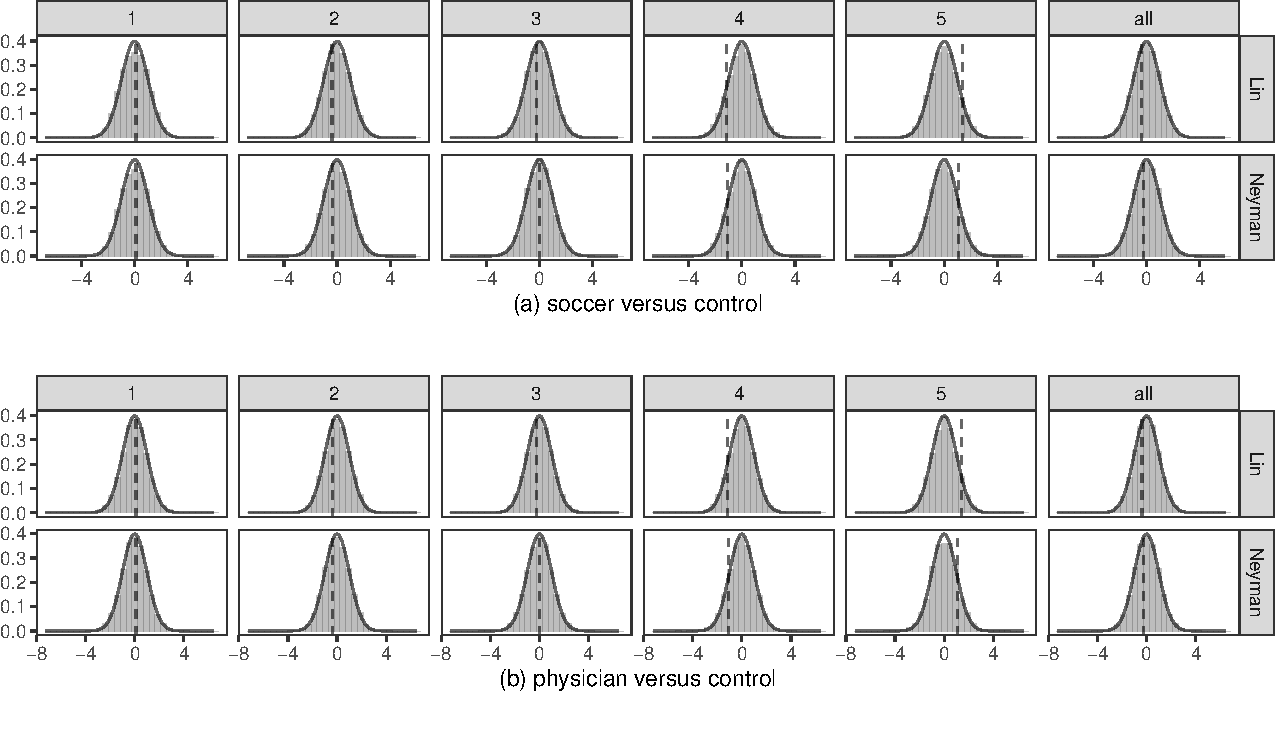
\includegraphics[width = \textwidth]{figures/frt_dist_chong.pdf}
\caption{\citet{chong2016iron}数据的再分析：含$5\times 10^4$次蒙特卡洛抽样的结果分布与$\N01$近似}
\label{fig::randomization-distributions-chong}
\end{sidewaysfigure}


 \section{作业习题}


\paragraph{重新分析\citet{angrist2009effects}的数据}\label{para::AL-mpe-fisher}

本题为内曼视角下的对应习题\ref{para::AL-mpe-neyman}。请计算各类学生化统计量对应的$p_\frt$值。 


\paragraph{复现\citet{zhao2020caFRT}的图1}\label{para::zhaoding-xfrt}

\citet{zhao2020caFRT}模拟比较不同统计量 FRT 的$p_\frt$有限样本性质，并根据图 1 推荐用$t_\textsc{L,S} $的 FRT 分析分层随机实验。请复现其图 1。 


\paragraph{推荐阅读}

在置换检验中使用学生化统计量并非新想法，参见\citet{Janssen97}和\citet{Romano13}。在基于设计的框架下，\citet{ding2017randomization}和\citet{wu2018randomization}针对多处理组实验提出了这一建议，\citet{zhao2020caFRT}将其推广到协变量调整。  

